\chapter{Supersonic flow over a wedge using OpenFOAM}
\thispagestyle{empty}
\label{sec:chap5}
\newcommand{\LocCHfivefig}{\Origin/CHAPTERS/chap5/figures}


In this chapter we would learn how to simulate a supersonic flow over a wedge and post-process it using ParaView. Here the domain for simulation is given as shown in fig \ref{geometry}$:$

\begin{figure}[ht]  
\begin{center}  
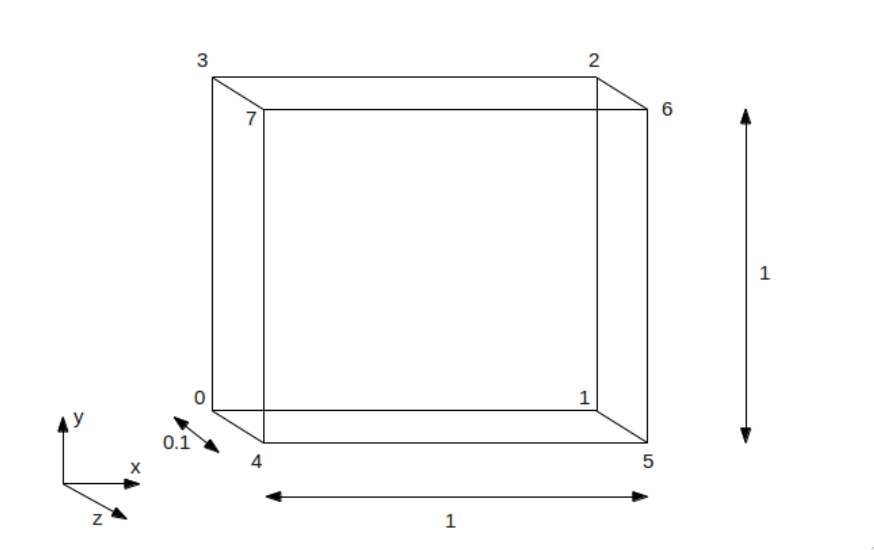
\includegraphics[scale=0.7]{\LocCHfivefig/geometry.png}
\caption{Geomtery of 2-D wedge along with boundary conditions}
\label{geometry}
\end{center}  
\end{figure}

\flushleft Please note that this chapter in written assuming the readers have some prior know on compressible flows and gas dynamics.

\flushleft As shown in the figure, in this problem statement we have a wedge at 15 degree with the horizontal and a flow from the inlet at 5 m/s. The boundary conditions used in the geometry file are similar to that as shown in the figure. Now this test case is already pready in the tutorial directory of OpenFoam. Thereby in this chapter we would mainly focus on how to simulate compressible flow over a given test case rather than creating a geometry. 
\flushleft Now to solve our present problem open acommand terminal by pressing $<$ctrl$>$, $<$Alt$>$ and $<$T$>$ simulataneously. After this enter the path for the current case file as shown below$:$
\flushleft cd run/tutorial/compressible/rhoCentralFoam/wedge15Ma5
\flushleft After openning the required case file enter 'ls'. This would show the folders within this case file. Here as mentioned in chapter 2 you would find three folders by the name$:$

\begin{itemize}
  \item 0
  \item constant
  \item system
\end{itemize}

\flushleft Now if you press 'cd 0' <enter> and then 'ls' $<$enter$>$ in the command terminal, you would find two folders given as:

\begin{itemize}
  \item P
  \item U
  \item T
\end{itemize}

\flushleft These folders gives the initial boundary conditions for pressure (i.e. P), velocity (i.e. U), temperature (i.e. T), etc of the geomtery. After this go back to the wedge folder by typing 'cd ..' $<$enter$>$.
\flushleft Now if you open the constant folder by entering 'cd constant' $<$enter$>$ in the command terminal followed by 'ls' <enter> you would find two folder$:$

\begin{itemize}
  \item polyMesh
  \item transportProperties
\end{itemize}

\flushleft Here polyMesh folder contains the blockMeshDict file. You can open this by typing 'cd poymesh' $<$enter$>$ followed by 'ls' $<$enter$>$ in the command terminal and then type 'gedit blockMeshDict'. This would show you the blockMeshDict file in text editor which contains the veritces, blocks and boundary patches of the geometry. The tranportProperties contain properties of the fluid medium used in this this problem. 
\flushleft Now you can go back to the wedge folder by entering cd .. twice in the command terminal. After this type 'cd system' <enter> followed by 'ls' $<$enter$>$. This would show you the three folders within system file.

\begin{itemize}
  \item ControlDict
  \item fvSchemes
  \item fvSolution
\end{itemize}


\flushleft Here controlDict file contains control parameters for start and stop of the number of iterations, fvSolution contain discretization schemes used for simualtion of this problem and fvSchemes contains equations for solver, tolerance, etc.
\flushleft To mesh the geometry go back to the cavity folder in the command terminal and enter the following and press $<$enter$>$$:$
\flushleft blockMesh
\flushleft This would mesh the geometry in a similar manner as shown in the previous chapter.If there are some error in the blockMesDict file, it would be shown in the command terminal. You can also type 'checkMesh' <enter> in the command terminal to check the different properties of the meshed geometry like number of cells, skewness, etc. 
\flushleft After this to view the meshed geometry, you can type 'paraFoam' $<$enter$>$ in the command terminal. This would open the ParaView window. Now on the ParaView window press apply on the left hand side of the Object Inspector Menu to view the meshed geometry. 

\begin{figure}[ht]  
\begin{center}  
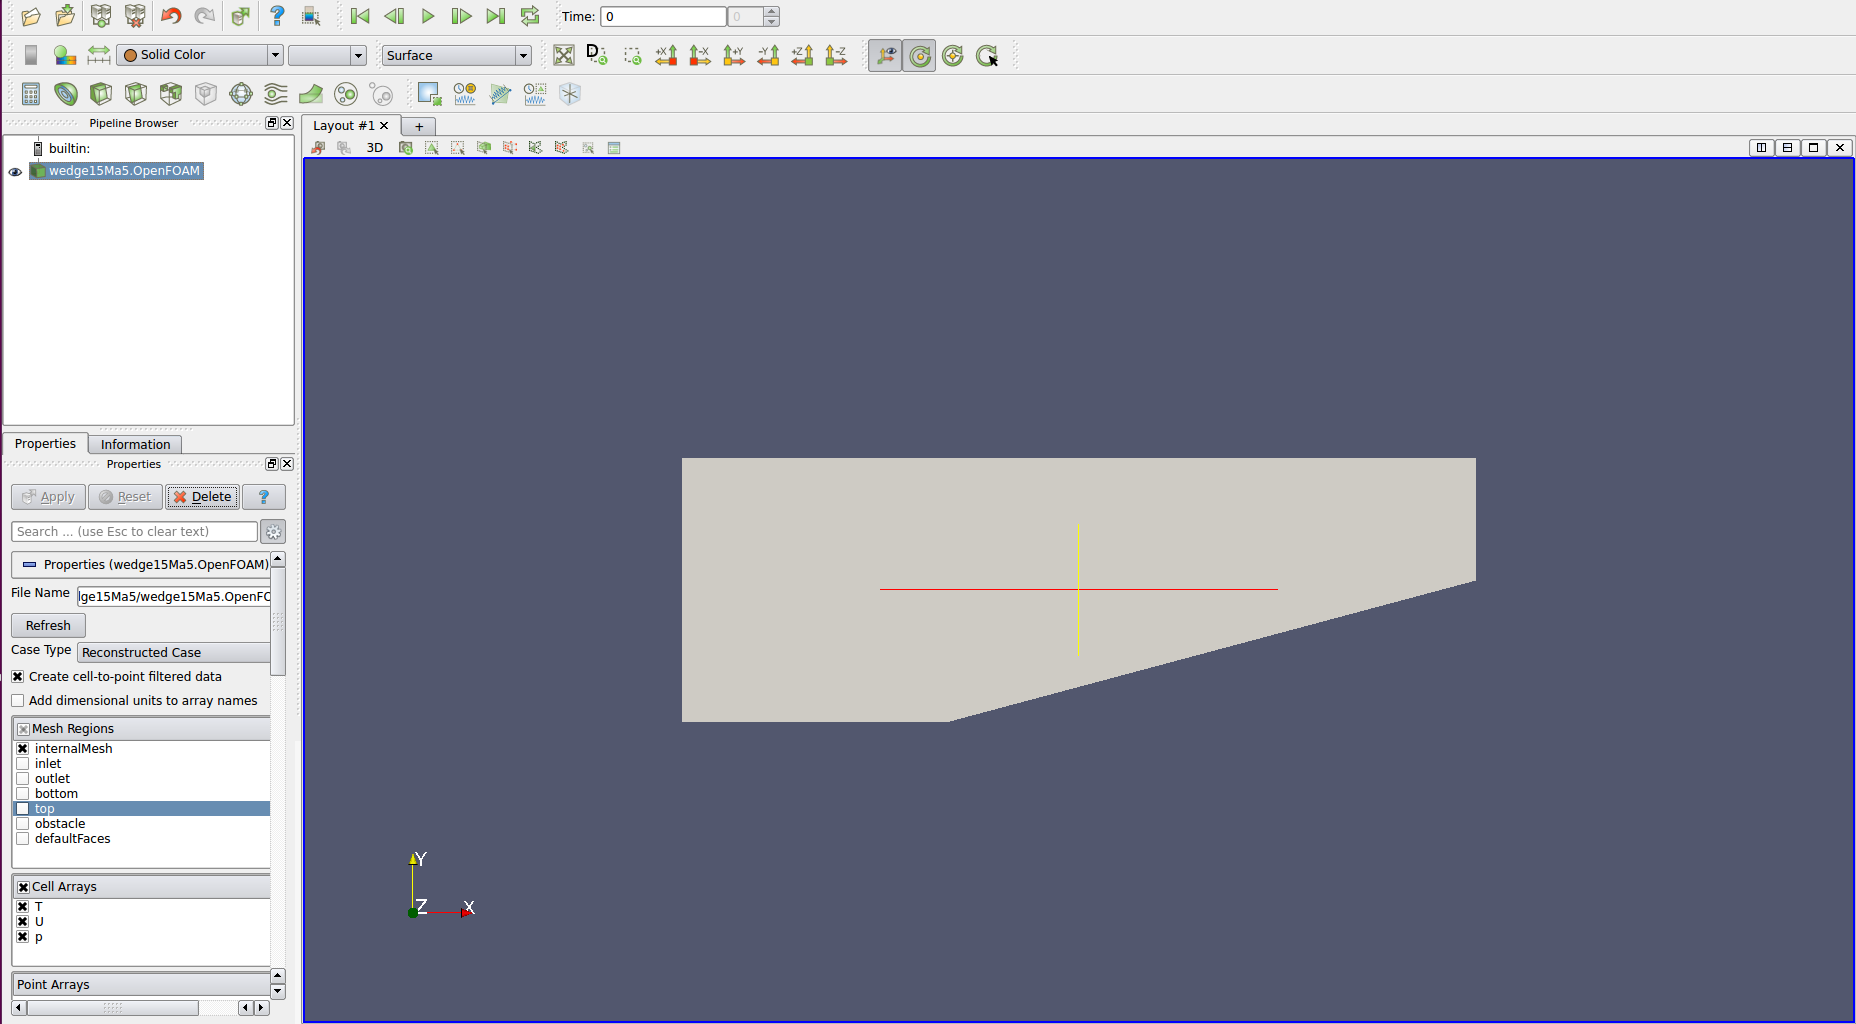
\includegraphics[scale=0.24]{\LocCHfivefig/para1.png}
\caption{Surface visualization of the 2-D wedge domain in ParaFView}
\label{para1}
\end{center}  
\end{figure}

\flushleft Now in the ParaView window you can check or uncheck the different regions within the 'mesh region' in  the Object Inspector Menu to visualize differnt regions on the geomtery. You can also visualize the geometry in wire-frame instead of surface by changing it from the down-down Active Variable Control Menu, to check out the quality of mesh.After inspecting the geomety you may close the ParaView window and switch back to the command terminal.

\begin{figure}[ht]  
\begin{center}  
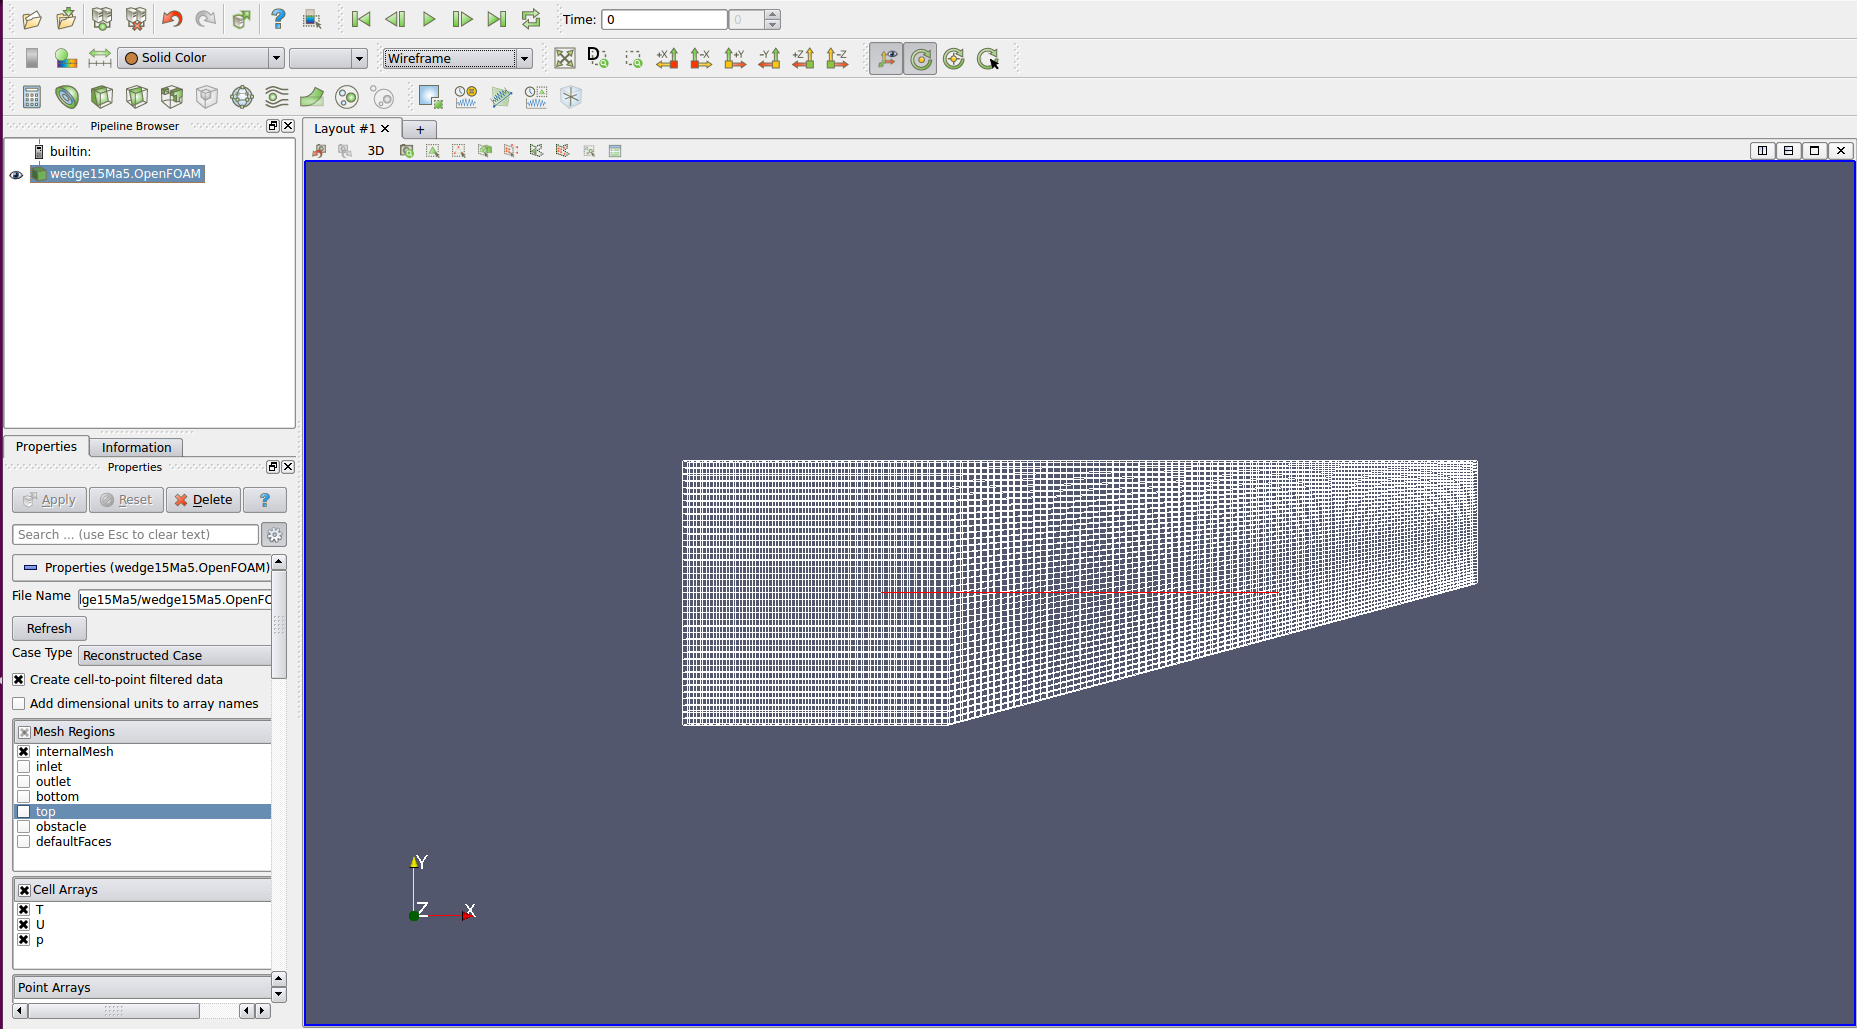
\includegraphics[scale=0.24]{\LocCHfivefig/para2.png}
\caption{Wireframe visualization of the 2-D wedge domain in ParaFView}
\label{para2}
\end{center}  
\end{figure}

\flushleft Now to run the solver switch back to the command terminal and type 'rhoCentralFoam' <enter>. The solver 'rhoCentralFoam' is a density-based compressible flow solver based on central-upwind schemes of Kurganov and Tadmor. You can see the progressing iterations in the terminal window along with the residual values. After the iteration ends type 'paraFoam' <enter> in the terminal window for post-processing.  
\flushleft This would open the ParaView window. As mentioned previously press apply on the left hand side of the Object Inspector Menu to view the new geometry. After this you can check or uncheck the different regions within the mesh region in  the Object Inspector Menu to visualize differnt regions on the geomtery. Now to check the velocity contours select U from the drop-down Active Variable Control Menu, from the visible toolbar. This will show the initial velocity countour of the cavity, as shown in fig \ref{velini}. Along with this you may also select the Toggle Colour Legend from the toolbar to visualize the legend. 

\begin{figure}[ht]  
\begin{center}  
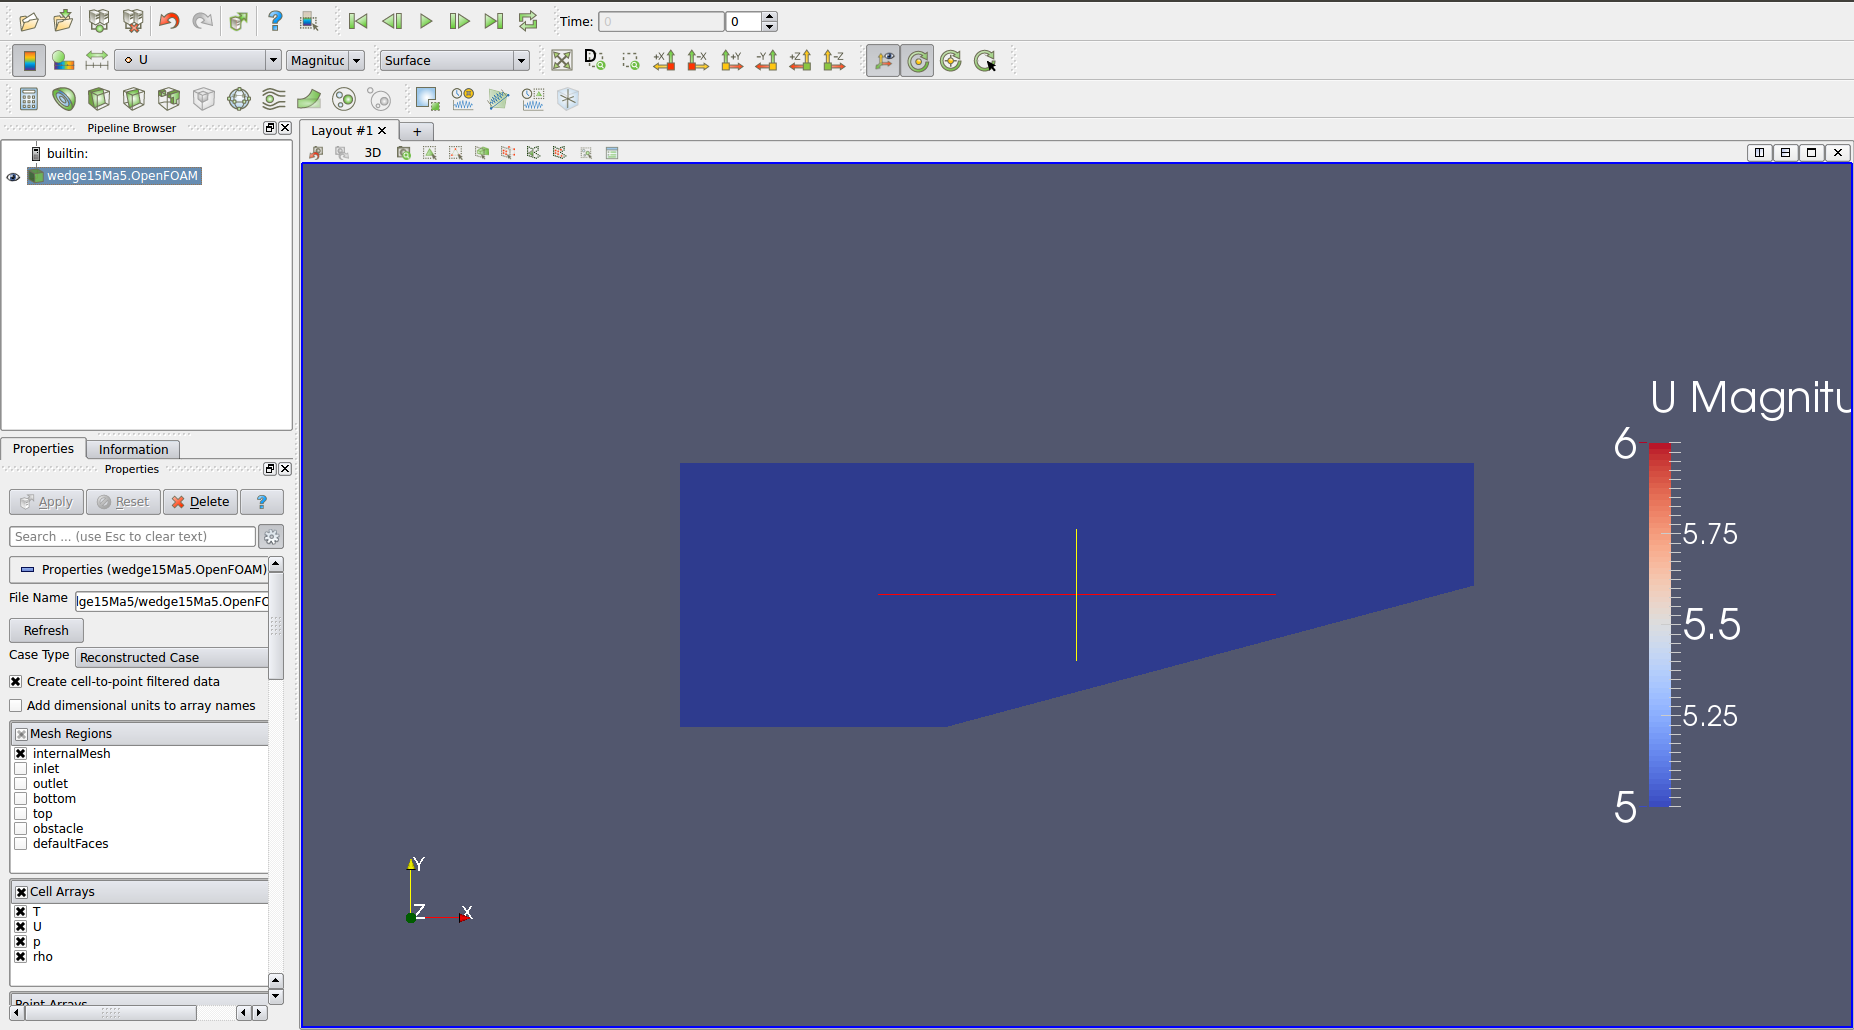
\includegraphics[scale=0.24]{\LocCHfivefig/velini.png}
\caption{Velocity contour in the 2-D wedge domain at initial state in ParaFView}
\label{velini}
\end{center}  
\end{figure}

\flushleft Now in the paraView window press the 'play' buttom from the VCR control. This would visualize the changing velocity countour along with the progressing iterations. You can see the final velocity contour as shown in fig \ref{vel}. Now on the ParaView window press apply on the left hand side of the Object Inspector Menu to view the meshed geometry. 

\begin{figure}[ht]  
\begin{center}  
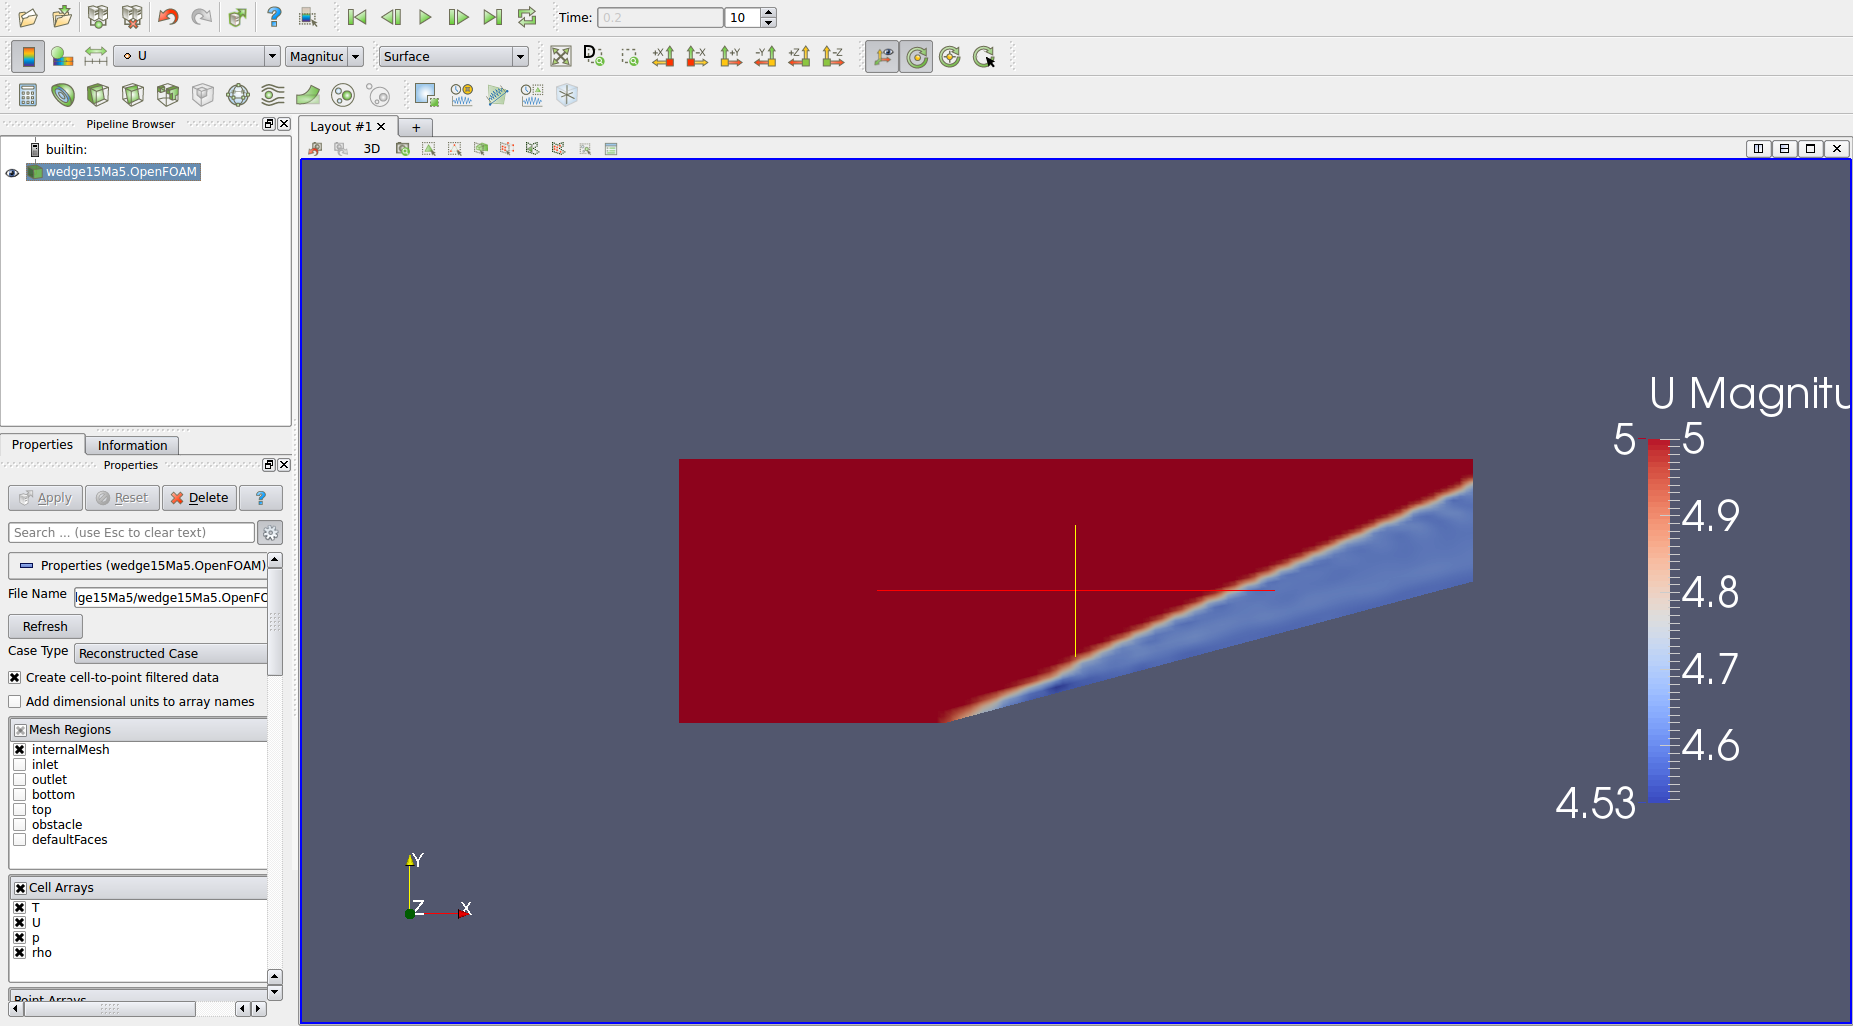
\includegraphics[scale=0.24]{\LocCHfivefig/vel.png}
\caption{Velocity contour in the 2-D wedge domain at final state in ParaFView}
\label{vel}
\end{center}  
\end{figure}

\flushleft Similarly, you can also plot the pressure and temperature contours.
\flushleft Now we can also calculate the mach number in this flow using a utility function in OpenFoam. To do this close the paraView window and switch to the command terminal. Here type 'Mach' and press $<$enter$>$. Note that “M” is capital here. This would calculate the Mach number in the flow for every time step.
\flushleft Now to view the Mach number contour type 'paraFoam' in the command terminal and press $<$enter$>$. Here select Mach in the left hand side properties window to include Mach number for post-processing. Now select 'Ma' from the drop-down Active Variable Control Menu, from the visible toolbar. And then press the play button on the VCR control toolbar. Along with this you may also select the Toggle Colour Legend from the toolbar to visualize the values to Mach number.
